\documentclass[11pt]{scrartcl}
\usepackage[sexy]{evan}

\begin{document}
\title{AM 220 HW 2}
\author{Haozhe (Stephen) Yang}
\date{\today}
\maketitle

\section{Problem 1}

\begin{enumerate}
    \item In matrix form, for all nodes, this can be written as:
    \[
    H^{(l+1)} = D^{-1} A H^{(l)},
    \]
    where $A$ is the adjacency matrix, $D$ is the degree matrix (the diagonal matrix with $D_{vv} = |\mathcal N_v|$), and \( H^{(l)} \) is the matrix of all node embeddings at layer \( l \).

    Here the $A H^{(l)}$ sums the neighbors of a node and then multiplication by $D^{-1}$ divides $|\mathcal N_v|$ at the front. Therefore, we see that the transition matrix $T$ is simply given by $T = D^{-1}A$, and so $H^{(l+1)} = TH^{(l)}$.
    \item When we modify the GNN, there's a $\frac 12$ chance of staying at the current place. So we see that \[H^{(l+1)} = \frac{1}{2} I H^{(l)} + \frac{1}{2} D^{-1} A H^{(l)} = \left( \frac{1}{2} I + \frac{1}{2} D^{-1} A \right) H^{(l)}.\]
    Therefore, the new transition matrix is \[T = \frac{1}{2} I + \frac{1}{2} D^{-1} A.\]
    Once again $H^{(l+1)} = TH^{(l)}$.
\end{enumerate}

\newpage

\section{Problem 2}

Note that at initialization, all nodes have input feature 0, except for the source node with input feature 1. At every iteration, nodes that are visited by BFS have embedding 1, and nodes that were not yet visited have embedding 0. To simulate BFS using a GNN, we can define the following:

\begin{itemize}
    \item \textbf{Aggregation function:} Each node aggregates incoming messages using a max operation. For node \(v\): \[m_v^{(l+1)} = f_{Agg}^{(l)}(h_v^{(l)}, \{h_u^{(l)}: u \in \mathcal N(v)\}) = \max\{h_u^{(l)}: u \in \mathcal N(v)\}\]
    This computes on step $l$ whether a neighbor of $v$ had been visited by the BFS algorithm.
    \item \textbf{Update rule:} A node updates its embedding to 1 if it is already visited or has a neighbor that is visited. That is:
    \[
    h_v^{(l+1)} = f_{up}^{(l)}\left(h_v^{(l)}, m_v^{(l+1)}\right) = \max\left(h_v^{(l)}, m_v^{(l+1)}\right)
    \]
    \item \textbf{Message function:} This is simply the message $m_v^{(l+1)}$, which records whether a neighbor of $v$ had been updated on the previous iteration.
\end{itemize}

This update rule mimics the layer-by-layer expansion of BFS: nodes directly connected to the source are updated in the first iteration, their neighbors in the next, and so on. Therefore, this GNN mimics the BFS algorithm.

\newpage

\section{Problem 3}

\begin{enumerate}[(a)]
    \item Note that because every node has value 1, regardless in which graph. When it is updated, all its neighbors has value 1, and so it's value will be updated to 1. Therefore, we see that every node value will remain at 1 after every update, regardless which graph it is. Thus, we see that regardless how many layers there are, the two nodes will always have the same embedding.
    \item Note that in class we have shown that GNNs are not more powerful then the 1-WL test. Therefore, to show that standard Message-Passing GNNs cannot learn these features of the graph, we simply come up with two graphs for each case to demonstrate that 1-WL test will give the same result: \begin{itemize}
        \item For the girth, As we saw in class for the following example: \begin{center}
            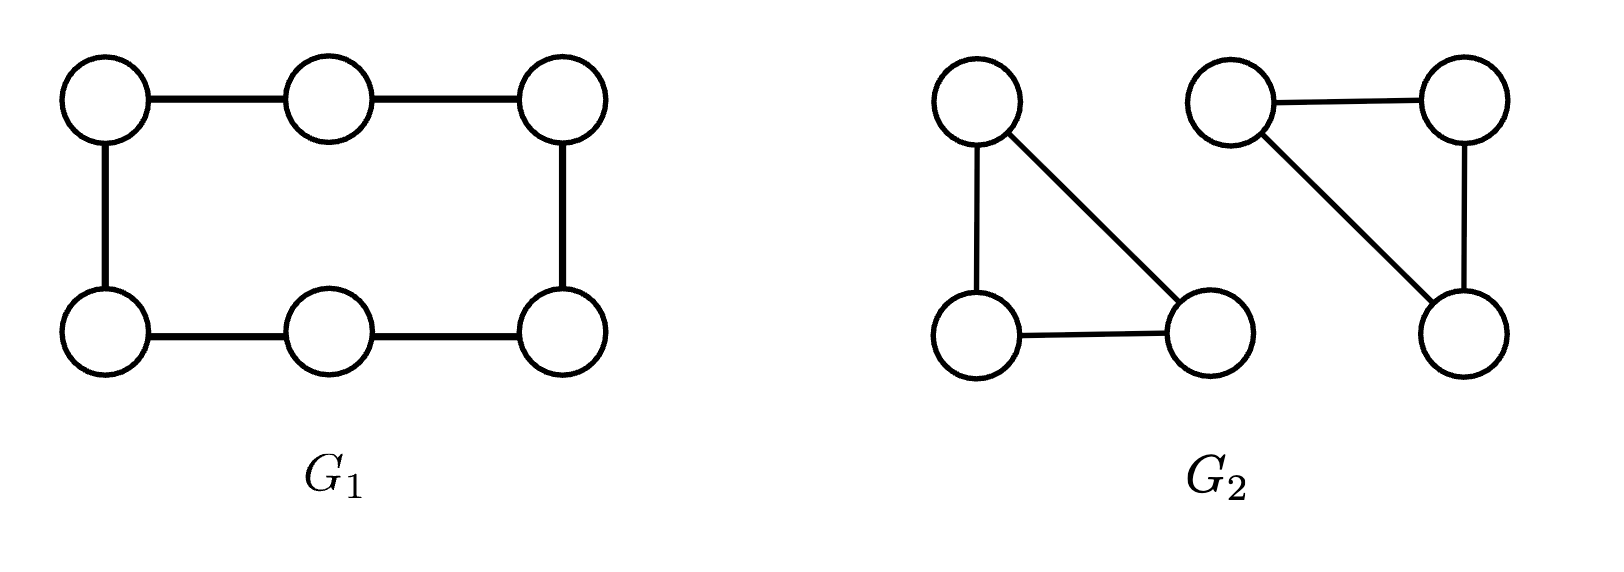
\includegraphics[width=12cm]{hw2-img/hw2-p3-b1.png}
        \end{center}
        We see that $G_1$ has girth 6 but $G_2$ has girth 3. However, the 1-WL test cannot distinguish these two graphs at all. Therefore, we see that basic MPGNN will not be able to distinguish these two graphs and hence cannot distinguish the girth of these two graphs.
        \item For the circumference, we can use the same example as above. The circumference of $G_1$ is 6, but the circumference of $G_2$ is 3. Again MPGNN cannot distinguish these two.
        \item Note that in lecture we have stated that 1-WL test cannot distinguish regular graphs. Therefore, we take two 3-regular graphs: \begin{center}
            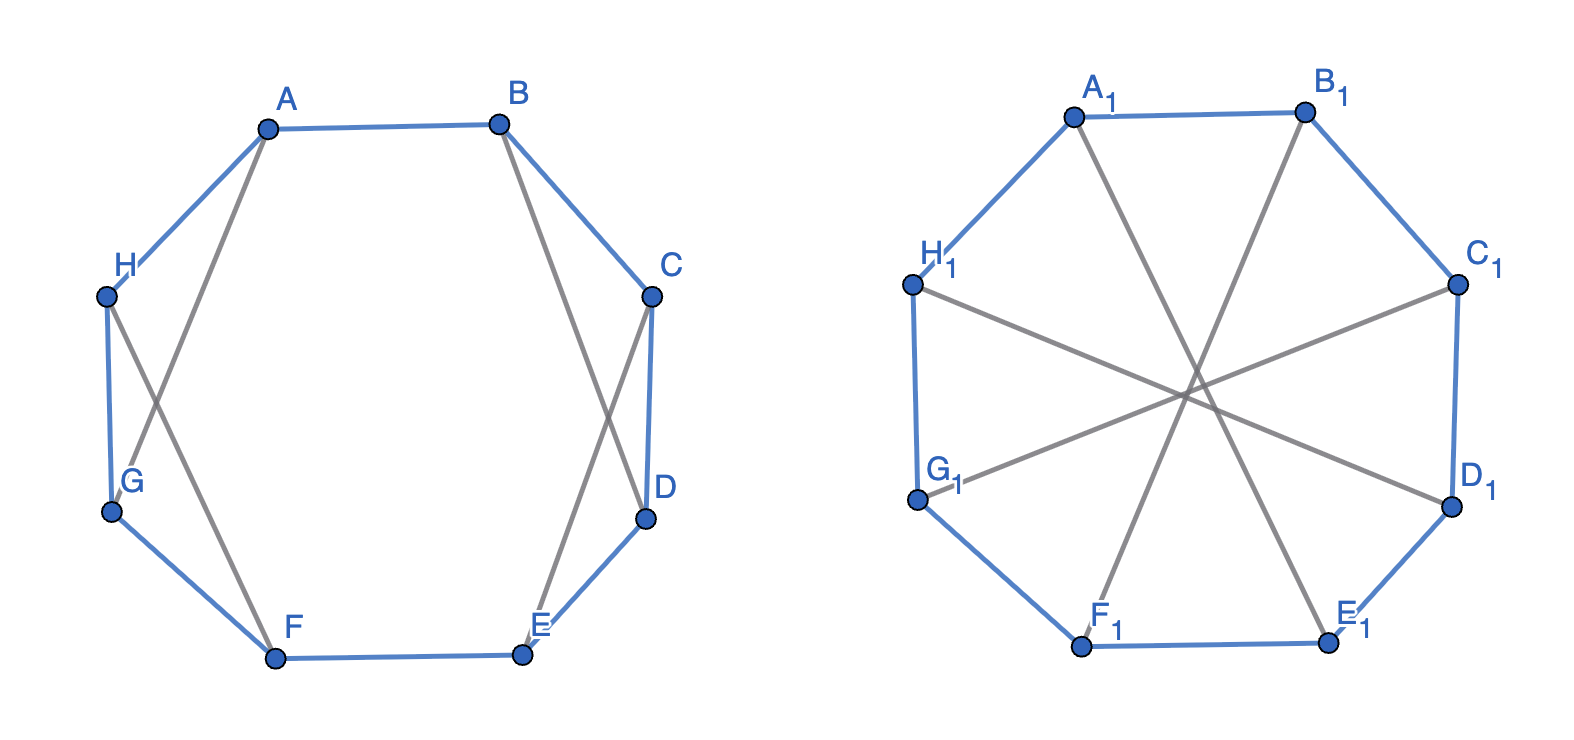
\includegraphics[width=12cm]{hw2-img/hw2-p3-b2.png}
        \end{center}
        Note that in the first graph, the longest distance is 3 (from $A$ to $E$). In the second graph, the longest distance is 2 (either by going across the diagonal or on the circumference). However, MPGNN cannot distinguish these two graphs. So we see that MPGNN cannot distinguish the diameter between the two graphs.
    \end{itemize}
    As such we see that MPGNNs cannot learn these characteristics.
    \item Note that in this case, define $\tilde D = I + D$, where $D$ is the degree matrix, and $\tilde A = I+A$, where $A$ is the adjacency matrix. Note that the update rule is $H^{(l+1)} = \tilde D^{-1}\tilde A H^{(l)}$. Therefore, based on the paper, we see that \[I_l(x, y) \propto \sum_{\text{all matrix entries}} \frac{\partial h_x^{(l)}}{\partial h_y^{(0)}}\]
    As $k$ increases, we see that this is some constant term multiplied by $(\tilde{D}^{-1}\tilde A)$ raised to $k$th power. 

    In particular, this represents the transition matrix of a lazy random walk. It is well know that a lazy random walk will eventually converge. For example, this \href{https://www.cs.yale.edu/homes/spielman/561/lect10-18.pdf}{Yale} handout gives a proof, which guarentees the random walk to converge to some stable distribution. It follows that the partial derivative rate of change for all $h_y^{(l)}$ wrt to $h_x^{(0)}$ as $l \to \infty$ will converge. Thus, we have that the node embeddings converges as $l \to \infty$.

    Finally, if we don't want the embedding to converge, we can alleviate this issue by using a shallow GNN. So that we terminate before the GNN converges. 
\end{enumerate}

\newpage

\section{Problem 4}

The Jupyter Notebook can be found on my GitHub: \href{https://github.com/haozheyang42/AM220-Homeworks/blob/main/hw2/hw2.ipynb}{https://github.com/haozheyang42/AM220-Homeworks/blob/main/hw2/hw2.ipynb}. I will also include code snippets in the pdf.

\begin{enumerate}[(a)]
    \item I used TSNE method to embed the dataset in 2d, here is the plot: \begin{center}
        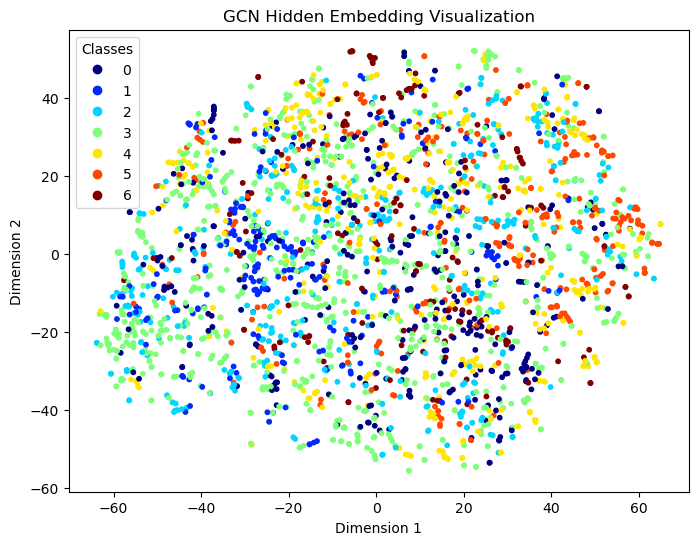
\includegraphics[width=10cm]{hw2-img/hw2-p4-a.png}
    \end{center}
    which is terrible, we cannot distinguish between clusters at all. The code that generated the plot is: \begin{verbatim}
    def plot(out):
        embeddings_2d = TSNE(n_components=2, random_state=42)
            .fit_transform(out.cpu().numpy())
        plt.figure(figsize=(8, 6))
        scatter = plt.scatter(embeddings_2d[:, 0], embeddings_2d[:, 1],
                              c=data.y.cpu().numpy(), cmap='jet', s=10)
        plt.legend(*scatter.legend_elements(), title="Classes")
        plt.title("GCN Hidden Embedding Visualization")
        plt.xlabel("Dimension 1")
        plt.ylabel("Dimension 2")
        plt.show()
    \end{verbatim}
    \item After training the model, we found the accuracy to be 0.8110, with the following test function: \begin{verbatim}
    def test():
        ##############################
        #  Implement a test function #
        ##############################
        model.eval()
        out = model(data.x, data.edge_index)
        pred = out.argmax(dim=1)
        
        mask = data.test_mask
        correct = pred[mask].eq(data.y[mask]).sum().item()
        acc = correct / mask.sum().item()
        return acc
    \end{verbatim}
    \item Using the same plot function as (a), we find the plot to be \begin{center}
        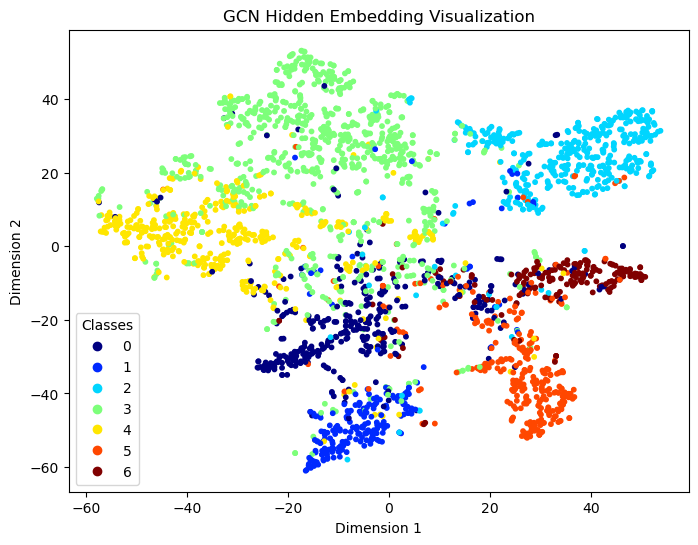
\includegraphics[width=10cm]{hw2-img/hw2-p4-c.png}
    \end{center}
    which is much better embedding than the part (a) untrained embedding. We can easily distinguish clusters in the data.
    \item By running the same method as before, we get the following plots: \begin{center}
        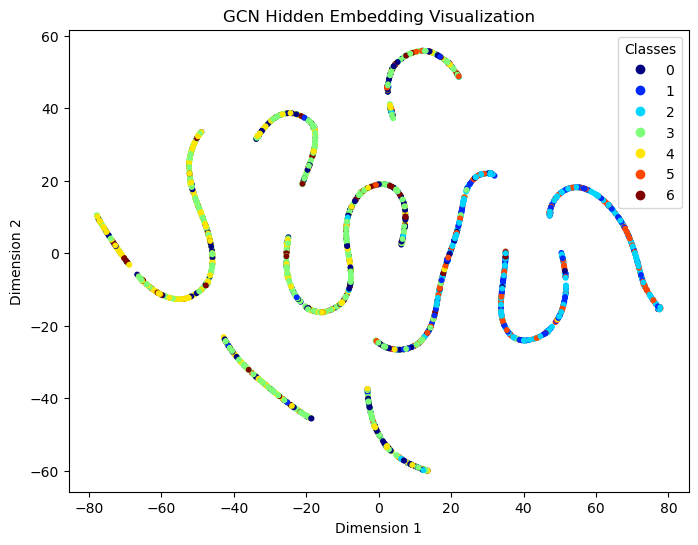
\includegraphics[width=6.5cm]{hw2-img/hw2-p4-d1.png}
        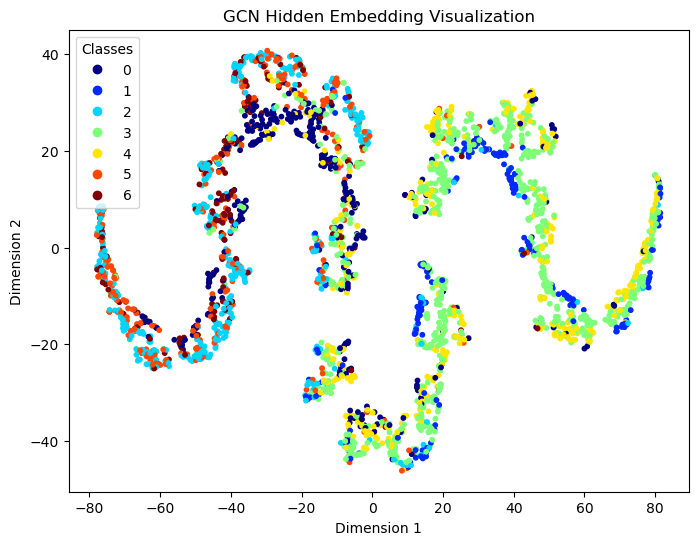
\includegraphics[width=6.5cm]{hw2-img/hw2-p4-d2.png}
        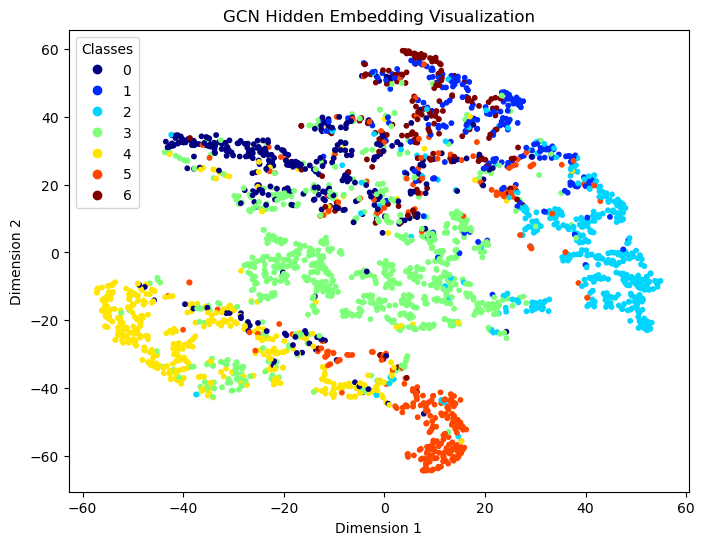
\includegraphics[width=6.5cm]{hw2-img/hw2-p4-d4.png}
        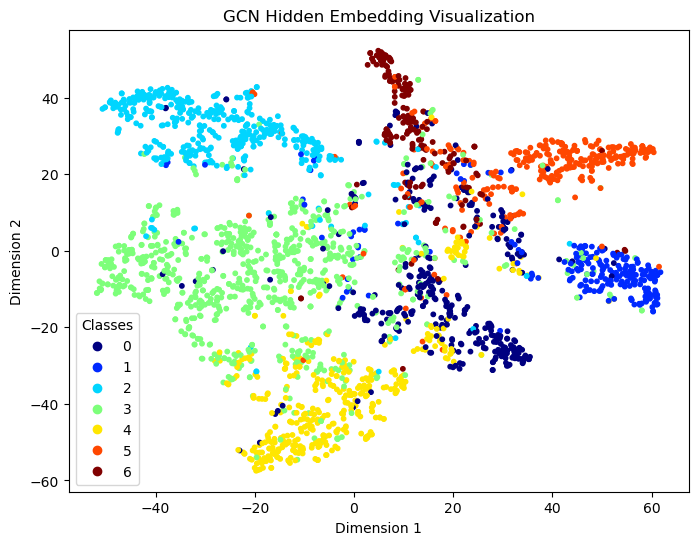
\includegraphics[width=6.5cm]{hw2-img/hw2-p4-d8.png}
        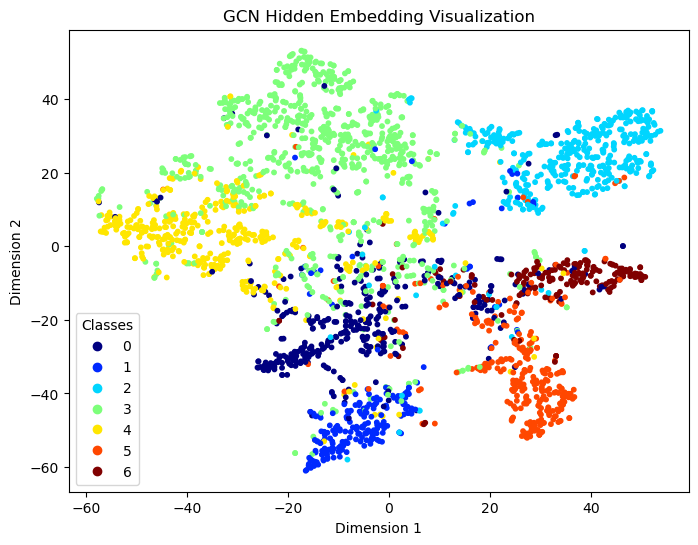
\includegraphics[width=6.5cm]{hw2-img/hw2-p4-d16.png}
        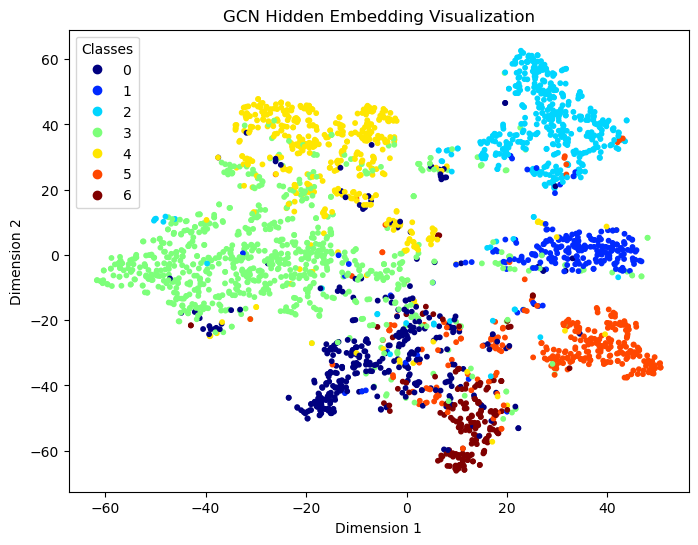
\includegraphics[width=6.5cm]{hw2-img/hw2-p4-d32.png}
        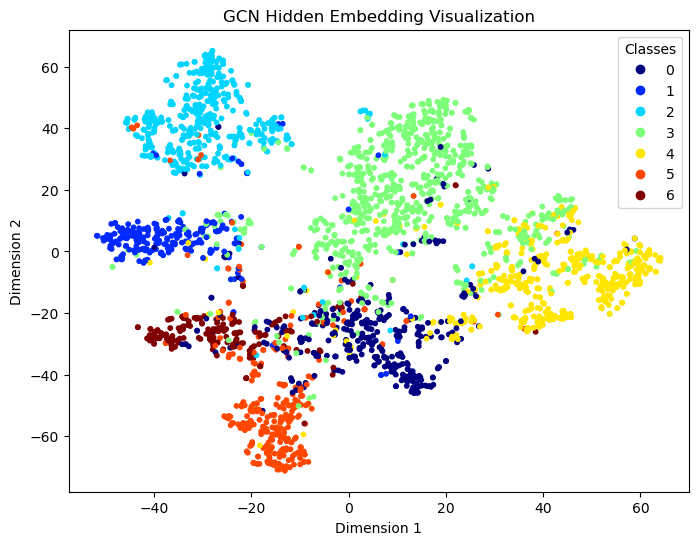
\includegraphics[width=6.5cm]{hw2-img/hw2-p4-d64.png}
    \end{center}
    The plots are for hidden feature dimensionality $=1, 2, 4, 8, 16, 32, 64$, respectively. We see that when hidden dimension is around 8, the embeddings are already quite good. But dimensions below 8 (less than the number of classes) gives really bad embeddings. I didn't include changing the number of layers, but it does not affect the result much.
    \item The following GCN class is implemented: \begin{verbatim}
    class GCN(torch.nn.Module):
        def __init__(self, hidden_channels):
            super(GCN, self).__init__()
            torch.manual_seed(12345)
            self.conv1 = GCNConv(dataset.num_node_features, hidden_channels)
            self.conv2 = GCNConv(hidden_channels, hidden_channels)
            self.conv3 = GCNConv(hidden_channels, hidden_channels)
            self.lin = Linear(hidden_channels, dataset.num_classes)
        
        def forward(self, x, edge_index, batch):
            # 1. Obtain node embeddings via GCN layers + ReLU activations
            x = self.conv1(x, edge_index)
            x = x.relu()
            x = self.conv2(x, edge_index)
            x = x.relu()
            x = self.conv3(x, edge_index)
            x = x.relu()

            # 2. Readout layer (global mean pool across nodes)
            x = global_mean_pool(x, batch)

            # 3. Final classifier
            x = self.lin(x)
            return F.softmax(x, dim=1)
    \end{verbatim}
    \item We checked its accuracy is ``Test Accuracy: 0.7368421052631579.''
    \item The following GNN class is implemented: \begin{verbatim}
    class GNN(torch.nn.Module):
        def __init__(self, hidden_channels):
            super(GNN, self).__init__()
            torch.manual_seed(12345)
            self.conv1 = GraphConv(dataset.num_node_features, hidden_channels) # Add your code
            self.conv2 = GraphConv(hidden_channels, hidden_channels) # Add your code
            self.conv3 = GraphConv(hidden_channels, hidden_channels) # Add your code
            self.lin = Linear(hidden_channels, dataset.num_classes)

        def forward(self, x, edge_index, batch):
            x = self.conv1(x, edge_index)
            x = x.relu()
            x = self.conv2(x, edge_index)
            x = x.relu()
            x = self.conv3(x, edge_index)

            x = global_mean_pool(x, batch)

            x = F.dropout(x, p=0.5, training=self.training)
            x = self.lin(x)
            
            return F.softmax(x, dim = 1)
    \end{verbatim}
    We checked its accuracy is ``Test Accuracy: 0.7894736842105263.'' Note that this is higher than before, which makes sense since the graph structure is more identifiable without the normalization.
\end{enumerate}

\end{document}